Jusque maintenant, le projet était une application unique mise en place chez le client.
Cette application comprenait le versionnage, le chiffrement, l'envoie des fichiers ainsi
que l'interface web.

L'hébergeur, montrant un certain intérêt pour le projet, a décidé d'héberger également
l'interface web. Le projet se présente donc de la manière suivante :

\begin{description}
     \item[Client:] Application de versionnage, de chiffrement et d'envoie des fichiers.
     \item[Hébergeur:] Application web.
\end{description}

Ainsi, il s'agit de développer un gestionnaire de version à notre sauce, j'entends par là :
indexer les fichiers, ne stocker que les différences, envoyer l'index et les fichiers sur un
serveur distant, ...

L'application web serait à ce logiciel ce qu'un \textbf{gitweb} est à \textit{git}.

\subsection{Architecture de l'application}

Lors d'une réunion, nous avons décidé d'organiser le projet de la manière suivante :

\begin{itemize}
     \item Les fichiers sont découpés en blocs de taille fixe.
     \item Chaque bloc est chiffré, puis compressé.
     \item Ce sont les blocs qui sont versionnés, ainsi que l'arborescence.
     \item Pour l'envoi et la réception des nouvelles versions, on développera une API.
     \item On n'utilise donc plus une base de données \textit{SQL} pour le versionnage, mais une base de données
     dans le système de fichiers.
     \item Pour la répartition des blocs sur le système de fichiers, on utilisera un serveur de \textbf{sharding}.
     \item Le tout reste développé en \textit{Python} et côté serveur on utilise toujours \textit{Django}.
\end{itemize}

Voici un schéma de l'architecture prévue :

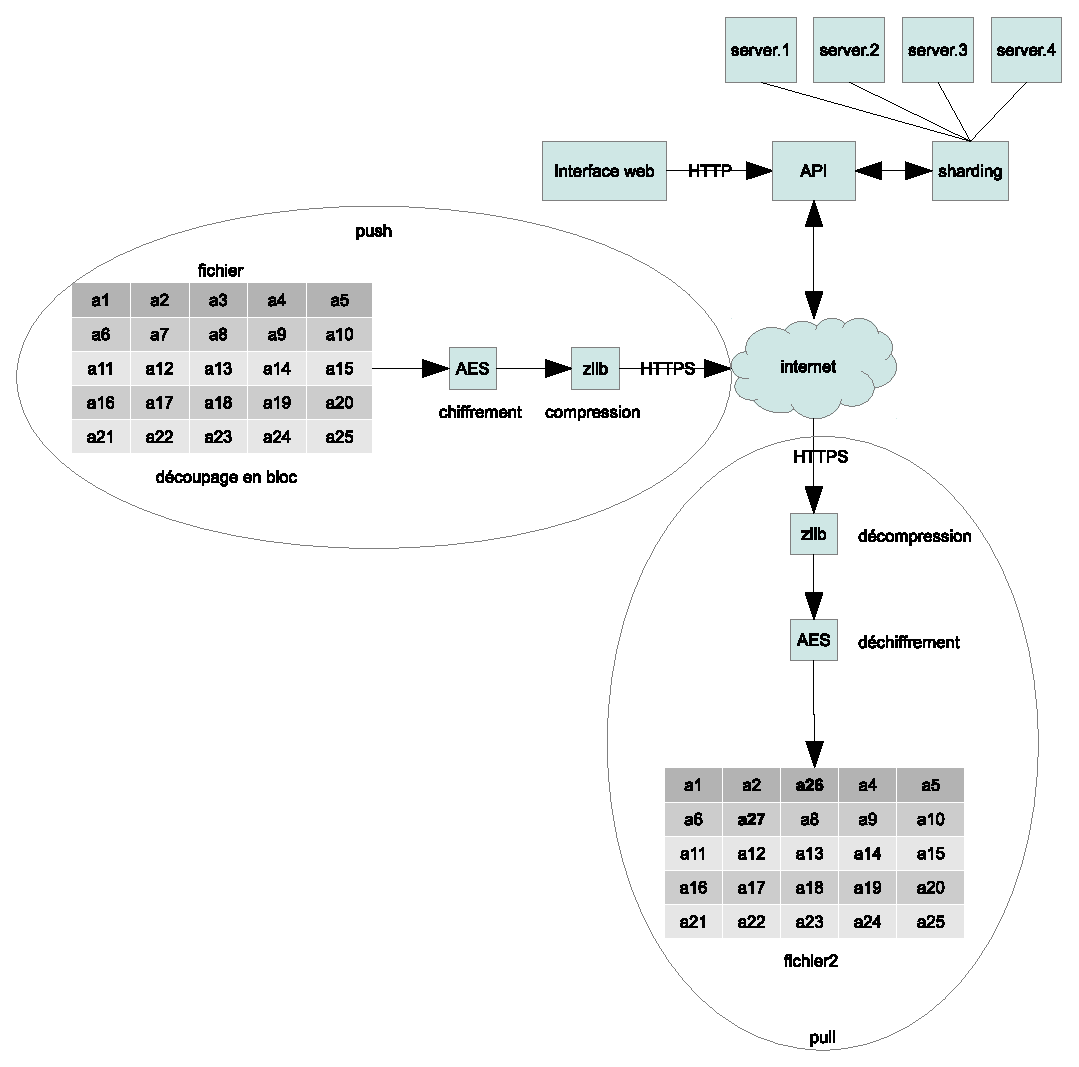
\includegraphics[scale=0.5]{img/architecture.eps}

\subsection{Présentation de l'API}

L'API sera donc utilisée pour envoyer ou recevoir de nouvelles versions, voici un exemple de ce que pourrait être l'API :

\subsubsection{Réception d'une nouvelle version}

\begin{verbatim}
GET /v1/{id client}/HEAD
     On récupère les meta-données de la révision d'arborescence.
     <==  {'HEAD': {'{id rev}': ['aefd475c', 'efda58b8', '1d25aecb', '548ef9d2', 'effda55c']}}

POST /v1/{id client}/{id rev}/files
     On envoie la liste des fichiers inconnus de notre révision locale.
     ==>  {'files': ['aefd457c', '548ef9d2']}
     On récupère la liste des blocs de chaque fichiers.
     <==  {'files': {
               'aefd457c': ['efda85e6', '8426efca', '422eda43', '45227d7e',
                            '9436d5ef', 'eadcb5e8'],
               '548ef9d2': ['aef475de', 'eefab5bc'],
               'blocksize': '4k'
          }}

POST /v1/{id client}/{id rev}/blocks
     On envoie la liste des blocs inconnus.
     ==>  {'blocks': ['efda85e6', '422eda43', '45227d7e', 'eadcb5e8', 'eefab5bc']}
     On récupère l'URL de chaque bloc.
     <==  {'blocks': {
               'efda85e6': 'http://sharding1.static.9h37.fr/ef/da/efda85e6',
               '422eda43': 'http://sharding3.static.9h37.fr/42/2e/422eda43',
               '45227d7e': 'http://sharding1.static.9h37.fr/45/22/45227d7e',
               'eadcb5e8': 'http://sharding2.static.9h37.fr/ea/dc/eadcb5e8',
               'eefab5bc': 'http://sharding1.static.9h37.fr/ee/fa/eefab5bc'
     }}
\end{verbatim}

\subsubsection{Envoi d'une nouvelle version}

\begin{verbatim}
POST /v1/{id client}/HEAD
     On envoie notre révision locale actuelle de l'arborescence.
     ==>  {'HEAD': {'{id rev local}': ['aefd475c', 'efda58b8', '1d25aecb',
                    '548ef9d2', 'effda55c']}}
     On récupère l'identifiant de la nouvelle version allouée.
     <==  {'HEAD': '{id rev remote}'}

POST /v1/{id client}/{id rev remote}/files
     On envoie la liste des fichiers
     ==>  {'files': {
               'aefd457c': ['efda85e6', '8426efca', '422eda43', '45227d7e',
                            '9436d5ef', 'eadcb5e8'],
               '548ef9d2': ['aef475de', 'eefab5bc'],
               'blocksize': '4k'
          }}
     Le serveur nous envoie la liste des blocs inconnus.
     <==  {'blocks': ['efda85e6', '422eda43', '45227d7e', 'eadcb5e8', 'eefab5bc']}

FOREACH block in blocks
     PUT /v1/{id client}/{id rev remote}/blocks/{id block}
          {DATA}
\end{verbatim}
